\mychapter{Teori}


\section{Kryptering}


\section{Blockchiffer}


\subsection{Körlägen}


\subsubsection{ECB}
\acrfull{ecb} är en av det enklaste blockchiffer körlägena som finns.
\acrshort{ecb} i sig är ganska lätt att förstå och bygger i huvudsak bara på
att man delar upp den data man vill kryptera i delar kallade block och tar sedan varje
block för sig och kör genom algoritmen, vilket tydligt visas i
figur \ref{fig:ecb-mode-enc} \& \ref{fig:ecb-mode-dec}.
\footfullcite{modesofoperation}

Figur \ref{fig:ecb-mode-enc} visar hur \acrshort{ecb} fungerar vid kryptering.
Här visas hur varje block för sig krypteras med hjälp av en blockchiffer algoritm
tillsammans med den givna nyckeln.

\begin{figure}[H]
    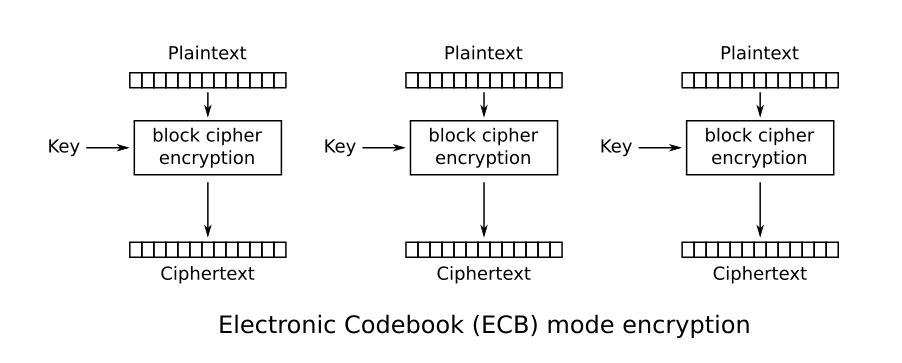
\includegraphics[width=\textwidth]{ECB_encryption.png}
    \caption{\acrlong{ecb} kryptering \cite{ecb-mode-enc-ref}}
    \label{fig:ecb-mode-enc}
\end{figure}

Figur \ref{fig:ecb-mode-dec} visar istället hur \acrshort{ecb} fungerar vid
dekryptering, vilken är en till stort sett identisk operation med det enda undantaget
att blockchiffret körs i dekrypterings läge istället för krypterings läge. % May need reformulating!!

\begin{figure}[H]
    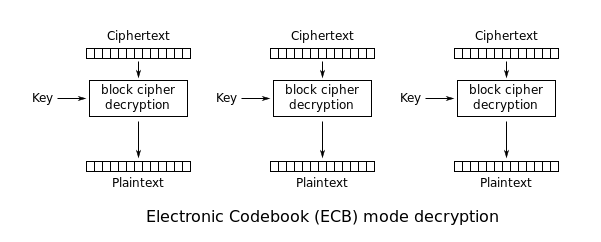
\includegraphics[width=\textwidth]{ECB_decryption.png}
    \caption{\acrlong{ecb} dekryptering \cite{ecb-mode-dec-ref}}
    \label{fig:ecb-mode-dec}
\end{figure}

På grund av \acrshort{ecb} körlägets simplicitet så finns det dock även ett ganska
stort problem med detta körläge. Det handlar om att \acrshort{ecb} inte på något
sätt förhindrar att två block med samma innehåll som krypteras inte resulterar i
ett identiskt krypterat block.\footcite{modesofoperation}

Vad detta innebär är att för större mängder data
är att det börjar bildas mönster i skiffertexten. Detta är något som väldigt
tydligt visar sig ifall man krypterar en bild, vilket går att se när man jämför
figur \ref{fig:pi-original} \& \ref{fig:pi-ecb}.
Det här faktumet är även varför \acrshort{ecb} inte är ett säkert körläge
och därför inte används näst intill aldrig i praktiken.\footcite{modesofoperation}

\subsubsection{CBC}
\acrlong{cbc} är ett av de mest vanligen använda körlägena för många blockchiffer.
Till skillnad från \acrshort{ecb} så förhindrar \acrshort{cbc} att två block med
samma innehåll kan ge samma krypterade block. Detta gör \acrshort{cbc} genom att
lägga till ett extra steg utöver vad som finns i \acrshort{ecb}. Steget
är en \gls{xor}-operation mellan det krypterade blocket nästkommande block innan
de körs genom blockchiffer algoritmen.\footcite{modesofoperation}
Matematisk sett kan detta formuleras såhär:

\begin{equation}
    \label{eq:cbc-encryption}
    \begin{aligned}
        &S_i = K_n(B_i \oplus S_{i-1})\\\nonumber
        &S_0 = IV
    \end{aligned}
\end{equation}

Där $S_i$ är det krypterade blocket(skiffertexten), $B_i$ är det blocket som ska krypteras,
$K_n$ är blockchiffer algoritmen där $n$ står för nyckeln och $S_{i-1}$ är
det krypterade blocket före det blocket som ska krypteras. \acrshort{iv} är en
\acrfull{iv} som används vid krypteringen av de första blocket då de inte finns
något föregående block att använda. $i$ står för index där de första blocket har
index värdet 1. Hela den här processen kan även ses i figur \ref{fig:cbc-mode-enc}.

\begin{figure}[H]
    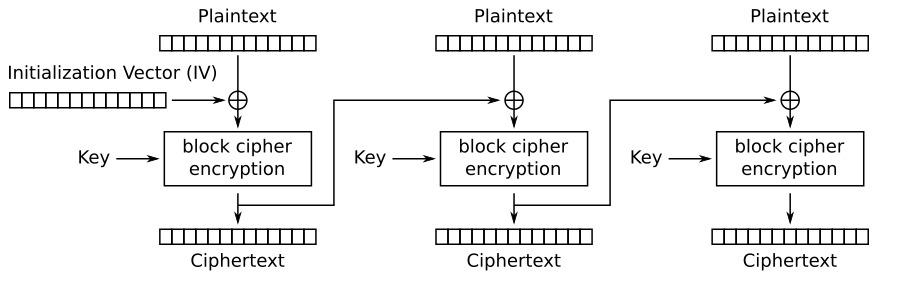
\includegraphics[width=\textwidth]{CBC_encryption.png}
    \caption{\acrlong{cbc} kryptering \cite{cbc-mode-enc-ref}}
    \label{fig:cbc-mode-enc}
\end{figure}

När de gäller dekrypterings processen för \acrshort{cbc} så bär den precis som för
\acrshort{ecb} stora likheter med krypterings processen. Det två skillnaderna som
finns är att blockchiffert körs i dekrypterings läge istället för krypterings läge.
Samt att för varje block så genomförs en \gls{xor}-operation mellan det dekrypterade
blocket och föregående block innan dekrypteringen av blocket.\footcite{modesofoperation}
Även detta går att både matematiskt formulera och visuellt visa såhär:

\begin{equation}
    \label{eq:cbc-decryption}
    \begin{aligned}
        &B_i = K_n(S_i) \oplus S_{i-1}\\\nonumber
        &S_0 = IV
    \end{aligned}
\end{equation}

\begin{figure}[H]
    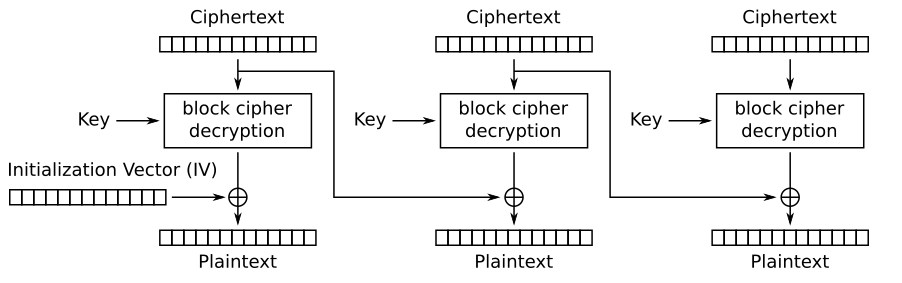
\includegraphics[width=\textwidth]{CBC_decryption.png}
    \caption{\acrlong{cbc} dekryptering \cite{cbc-mode-dec-ref}}
    \label{fig:cbc-mode-dec}
\end{figure}

Fördelarna som kommer från den extra operationen i \acrshort{cbc} till skillnad
från \acrshort{ecb} är då att varje block blir beroende av föregående block.
Detta innebär att möjliga mönster som kunde dyka upp i \acrshort{ecb} inte längre
kan uppstå, vilket då gör \acrshort{cbc} till ett säkrare körläge än \acrshort{ecb}.
Dock kräver cbc en ytterligare faktor för att se till så att inte olika medelanden
kan ge samma krypterade block. Därav så krävs en \acrfull{iv} som används vid första
blocket.\footcite{modesofoperation}

\acrshort{cbc} är dock inte prefekt och har i sig också några nackdelar. Bland dessa
så ... % TODO: skriv om detta
% pros: can be parallelized, no need to store previous block as well as IV
% IV can bee discarded if you use a random block as the first block in the message...
\footcite{modesofoperation}

\subsubsection{OFB}


\section{Symetrisk \& Asymmetrisk Kryptering}
Symetrisk och asymetrisk kryptering handlar om hur nycklar används i olika
krypteringsalgoritmer. För symetriska krypterings algoritmer så betyder detta
att samma nyckel är vad som används för både kryptering och dekryptering.

\footfullcite{symencrypt}

\section{AES}


\subsection{Finite Fields}


\subsection{AES S-Box}


\subsection{Struktur}


\subsubsection{SubBytes operation}
SubBytes operationen bygger på ...

\subsubsection{ShiftRows operation}


\subsubsection{MixColumns operation}


\subsubsection{AddRoundKey operation}


\subsection{Nyckel utökning}


\subsubsection{RotWord}


\subsubsection{SubWord}


\subsubsection{Rcon}


\subsection{AES-128bit}


\subsection{AES-192bit}


\subsection{AES-256bit}

